% !TEX root = ../main.tex
\section{Findings for the Entire Population}

	\subsection{Pattern Creation Time}
		\begin{figure}[H]
      \subfigure[Average pattern creation time (seconds)]{
        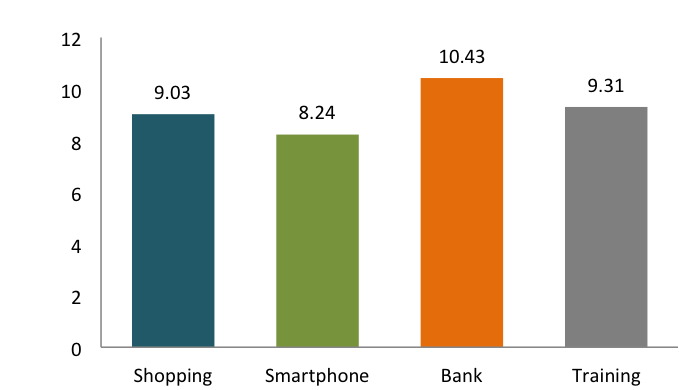
\includegraphics[scale=0.48]{pics/analysis/avgCreationTime.png}
      }
      \subfigure[Creation time and experience with ALP]{
        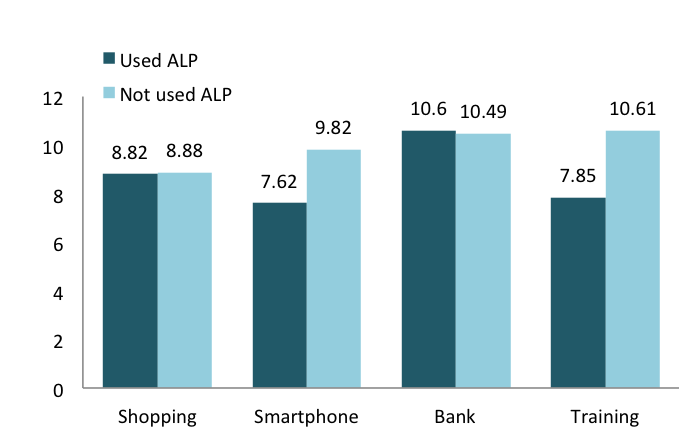
\includegraphics[width=0.48\textwidth]{pics/analysis/usedALPpatterncreationtime2.png}
      }
      \caption{Pattern creation time for the entire population}
    \end{figure}

	\subsection{Pattern Length}

		\begin{figure}[H]
      \centering
      \subfigure[Average Pattern Length (nodes)]{
        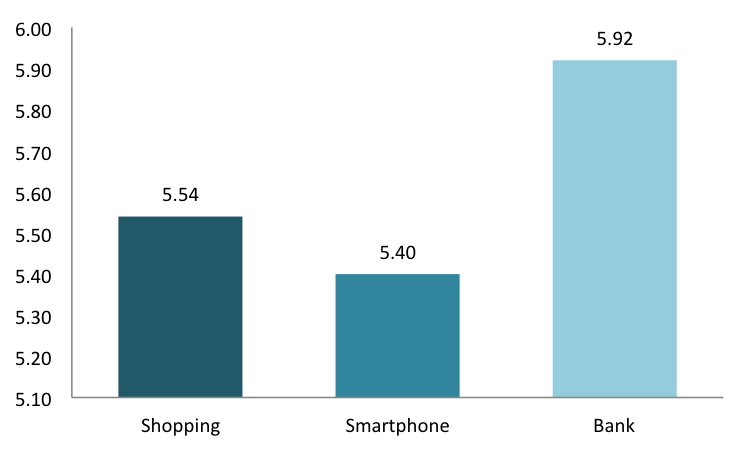
\includegraphics[scale=0.48]{pics/analysis/avgPatternLength.png}
      }
      \subfigure[Pattern length distribution]{
        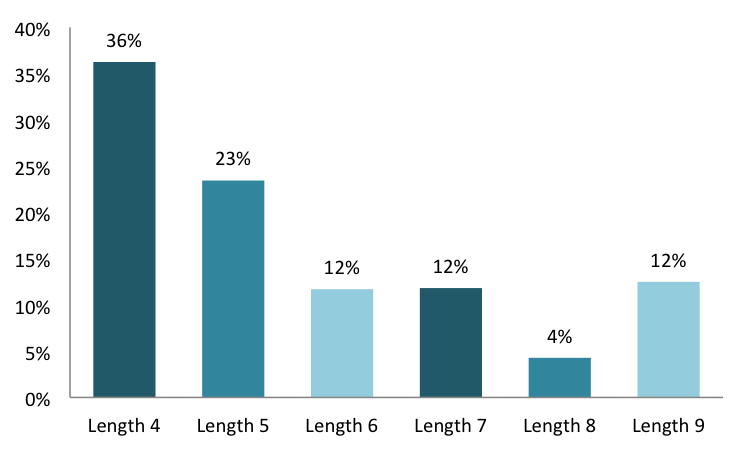
\includegraphics[width=0.48\textwidth]{pics/analysis/patternLength.png}
      }
      \caption{Pattern Length for the entire population}
    \end{figure}

		%Figure:Pattern length and type distribution
    \begin{figure}[H]
      \centering
      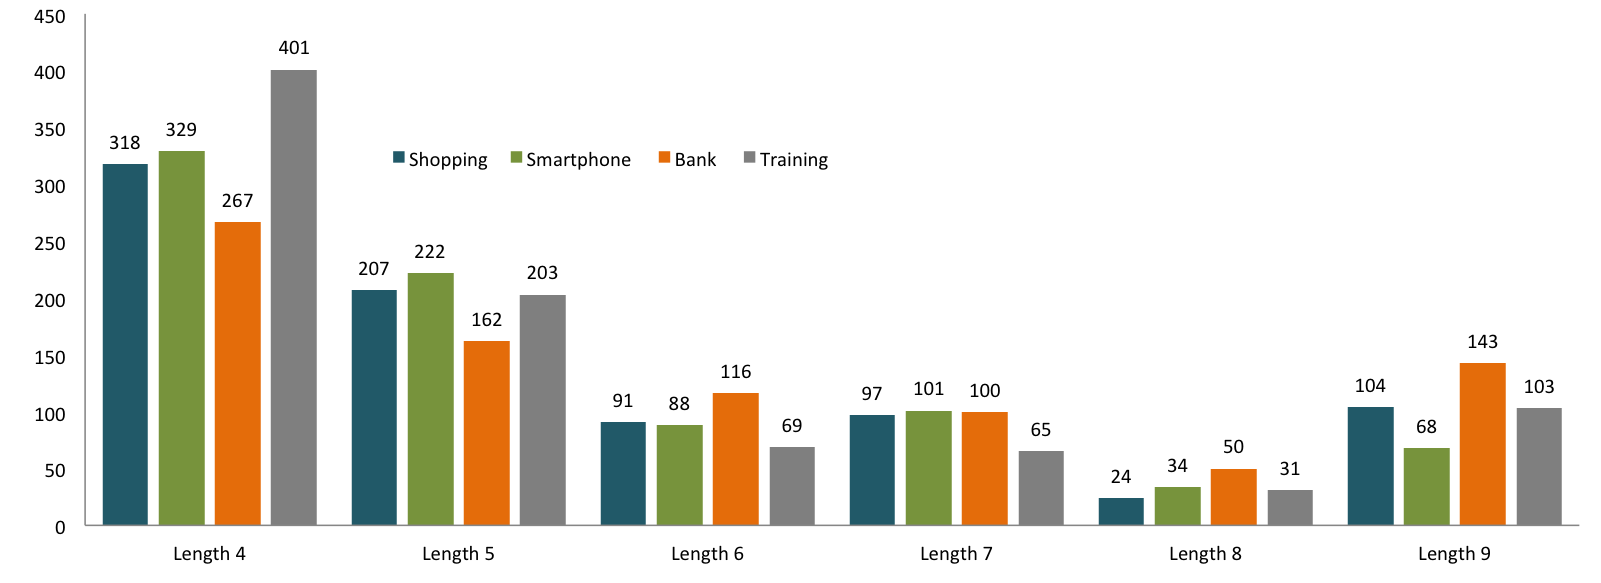
\includegraphics[width=\textwidth]{pics/analysis/patterntypePatternLength.png}
      \caption{Pattern length and type distribution}
      \label{fig:patternTypePatternLength}
    \end{figure}


	\subsection{Pattern Complexity}

		\begin{table}[H]
      \begin{tabular}{l || l | l | l | l || l}
        \hline
        {\bf Parameters} & {\bf Shopping} & {\bf Smartphone} & {\bf Bank} & {\bf Training} & {\bf All} \\ \hline
        \#Patterns & 841 & 842 & 838 & 872 & 3393 \\
        Avg. Size & 5.541 & 5.398 & 5.920 & 5.347 & 5.549 \\ 
        Avg. Length & 5.050 & 4.920 & 5.666 & 47886 & 5.103 \\
        \#Intersections & 177 & 149 & 363 & 143 & 832 \\
        Avg. Intersections & 0.210 & 0.1769 & 0.433 & 0.16399 & 0.245 \\
        \#Overlaps & 15 & 12 & 19 & 9 & 55 \\
        Avg. Overlaps & 0.0178 & 0.014 & 0.023 & 0.010 & 0.016\\ \hline
        Avg. Strength & 13.440 & 12.837 & 15.514 & 12.545 & 13.572 \\ 
        Min strength & 6.339 & 6.339 & 6.339 & 6.339 & 6.339 \\
        Max strength & 44.441 & 43.187 & 44.441 & 43.187 & 44.441 \\ \hline
      \end{tabular}
      \caption{Pattern strength for all patterns types in the entire population}
      \label{tab:patternstrength}
    \end{table}

	\subsection{Pattern Characteristics}

		\todo[inline, color=blue!60]{Sette inn association elements? Dette er en karakteristikk som befinner seg på tvers av populasjonen}

		\todo[inline, color=blue!60]{Sette inn noe om startpunkt?}

		\todo[inline, color=blue!60]{Passer 3-gram inn her?}

		%Figure: Number of unique patterns
    \begin{figure}[H]
      \centering
      \begin{minipage}[b]{0.40\linewidth}
      \centering
        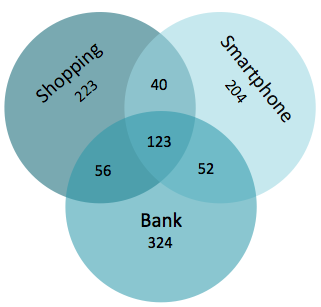
\includegraphics[scale=0.4]{pics/analysis/uniquePatternsVenn.png}
      \end{minipage}%
      \begin{minipage}[b]{0.30\linewidth}
        \centering
        \begin{tabular}{ c | c }
          \hline
          Shopping &  442 \\
          Smartphone & 419 \\
          Bank & 555 \\
          Training & 414 \\ \hline \hline
          All types & 1196 \\ \hline
        \end{tabular}
        \vspace{1cm}
      \end{minipage}
      \caption{Number of unique patterns}
      \label{fig:test}
    \end{figure}
